% \begin{wrapfigure}{l}{0.4\textwidth}        
\begin{center}
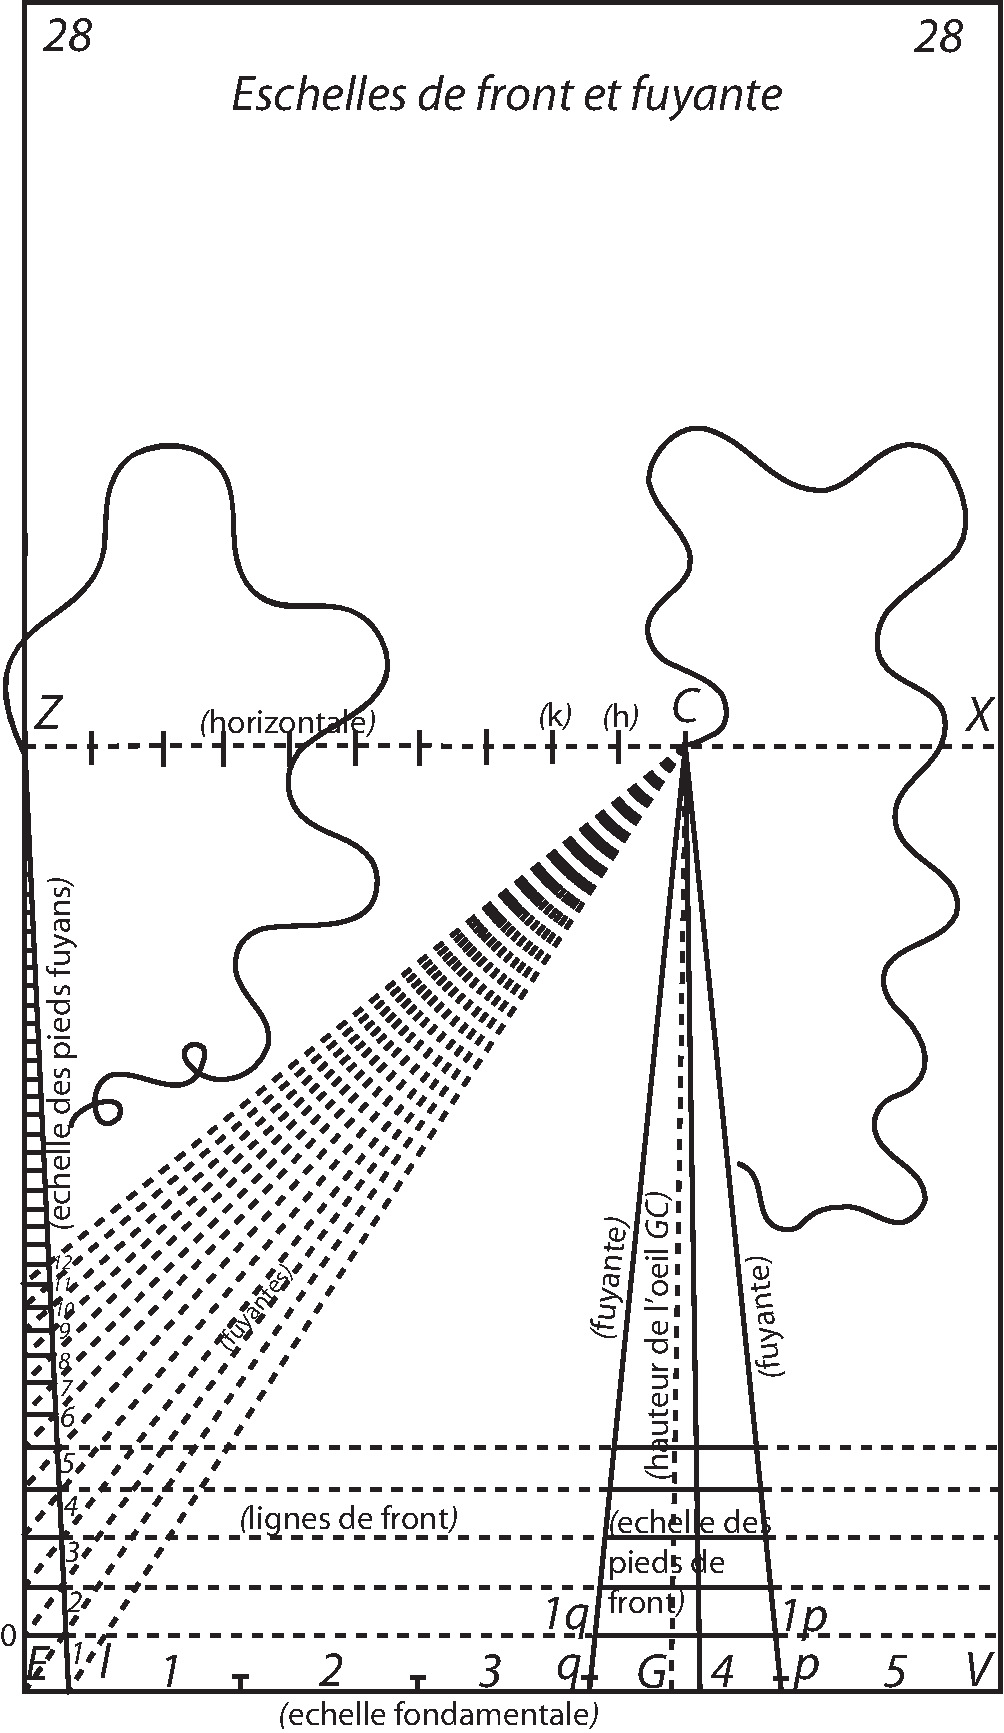
\includegraphics[width=0.6\textwidth]{images/T28-Desargues}\\\rule[-4mm]{0mm}{10mm}\textit{[Fig. 11]}\textsuperscript{10}
\end{center}
% \footnote}
\footnoterule % \vspace{2.0ex}\hspace{-0.7cm}\rule{1.8cm}{0.5pt}
\pstart\hspace{-10pt}\textsuperscript{10}\textit{Unter der \"{U}berschrift}: \textso{Pieds de front} sont les parties des lignes de front; comprises entre deux fuyantes\protect\index{Sachverzeichnis}{\'{e}chelle!fuyante} men\'{e}es des deux bouts \textit{q}, \textit{p} d'un pied de
\\
\footnoterule\\
l'echelle\protect\index{Sachverzeichnis}{\'{e}chelle} fondamentale \textit{EV} \`{a} un point \textit{C} de la ligne horizontale; \textit{ZX}.\textso{ L'echelle}\protect\index{Sachverzeichnis}{\'{e}chelle!de front} de front est la suite des pieds de front compris entre deux mêmes fuyantes. Prenez dans l'echelle\protect\index{Sachverzeichnis}{\'{e}chelle} fondamentale, une droite \textit{EL}, qui est \`{a} un pied de l'echelle\protect\index{Sachverzeichnis}{\'{e}chelle} fondamentale \textit{qp} comme \textit{CZ} prise dans l'horizontale depuis le point \textit{C}, est \`{a} la distance de la station \`{a} la conduite de front. Men\'{e}s \textit{EZ}, \textit{lZ } les parties des lignes de front, comprises entre les deux fuyantes \textit{EZ}, \textit{lZ} seront les pieds fuyans et leur suite sera l'echelle\protect\index{Sachverzeichnis}{\'{e}chelle} des pieds fuyans.\\ \textit{In der Mitte unter der Geraden}: \textit{ZX}: \textit{ch}, \textit{hk}, etc. \'{e}gal \`{a} \textit{El}\\ \textit{Links unter der Geraden}: \textit{ZX}: \textit{CZ} est autant de fois \textit{El} que la distance de la station \`{a} la conduite de front, a des pieds de long.\\ \textit{Unter der Zeichnung links}: \textit{El}\textso{ pied fuyans fondamental.} \textit{NB}\\ \textit{Unter der Zeichnung}: Suppose \textit{ZE} parallele \`{a} \textit{CG} il se demontre que \textit{EO} est egale \`{a} \textit{1q1p} car \textit{EO} : \textit{ZO} :: \textit{El} : \textit{GE} :: \textit{qp} : \textit{CZ} :: \textit{1q1p} : \textit{ZO}. La figure est mal faite, car \textit{CZ} deuuroit estre \`{a} \textit{CG} comme \textit{El} \`{a} \textit{qp}, et les deux premiers estans faits quasi egaux. Les derniers le deuuroient estre \edtext{aussi. \selectlanguage{latin} }{\lemma{aussi.}\Afootnote{\textbar\ supposant \textit{ZE} et \textit{CG} item \textit{CZ} et \textit{lE} paralleles et egales \textit{ gestr.}\ \textbar\ \ \ \ \textit{L}}}\\ \textit{Unter der Zeichnung rechts}: \textso{pied de front fondamental} NB, et \textso{pied geometral} NB sont une même chose \textit{qp}.\\ \textit{Neben der Zeichnung rechts am Rand}: \textit{CG} hauteur de l'oeil \textit{qp} pied \edtext{geometral \textit{El}}{\lemma{geometral}\Afootnote{ \textbar\ egal si vous voul\'{e}s \`{a} \textit{pq} \textit{ gestr.}\ \textbar\ \textit{El}\ \textit{L}\hspace{6cm}}} pris \`{a} discretion\\
\protect\begin{tabular}{l}$CZ:CG::EL:qp$\\$EG\hspace{9pt}CZ$\protect\end{tabular}\\\textit{EO} : \textit{O1} :: \textit{EZ} : \textit{CZ} :: \textit{qp} : \textit{El}\textit{ZO} : \textit{O1} :: \textit{ZE} : \textit{El} \\\rule[-4mm]{0mm}{10mm} $\protect\overbrace{\frac{ZE\cdot EI}{qp}}^{E0\cdot CZ}\protect\overbrace{ZE - E0}^{\sqcap\hspace{5pt} Z0\hspace{5pt}EI}$ \\seu \textit{ZO} : \textit{EO} :: \textit{GE} : \textit{El}. Ergo $\displaystyle 1\sqcap\frac{CG}{E0} - \frac{CG}{qp}$ seu $\displaystyle E0\; \sqcap \frac{CG\cdot qp}{CG+qp}$ \\itaque \textit{EO} prodit eadem, qualiscunque sumatur \textit{El} $\displaystyle CZ \sqcap \frac{CG \cdot El}{qp}$\rule[-4mm]{0mm}{10mm} 
\pend \addtocounter{footnote}{1}
          